\chapter*{Appendix A: Kontrolinterface}
I dette appendix vil jeg gå nærmere ind på opbygningen af den grafiske brugergrænseflade på Kontrolinterfacet.

\section*{Hovedvindue}
Det første vindue man ser ved programopstart er hovedvinduet, som vist på 
\begin{figure}[H]
\centering
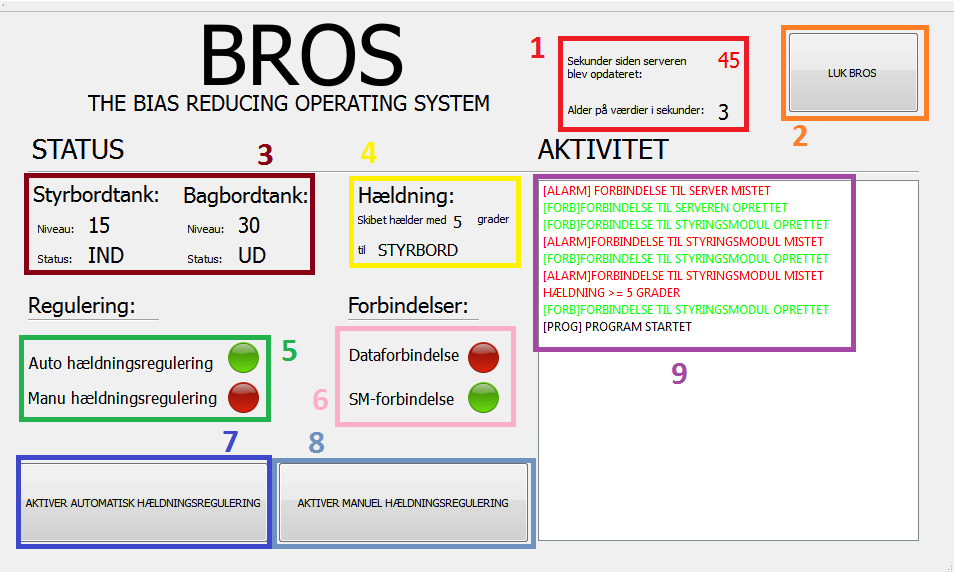
\includegraphics[width=1\textwidth]{billeder/GUI/hovedvindue_3_2}
\label{fig:hovedvindue}
\caption{På figuren ses hovedvinduet for Kontrolinterface-programmet}
\end{figure}


\begin{table}[H]
\begin{center}

\rowcolors{1}{white}{light-gray}
\begin{tabular}{| l | p{9.5cm} | }

\multicolumn{2}{l}{Hovedvinduets elementer} \\
\hline
\textcolor{red}{\textbf{1: Forsinkelse i sekunder}}
&Det øverste tal fortæller tiden i sekunder siden serveren sidst er blevet opdateret succesfuldt.
Nedenunder udskrives tiden i sekunder siden værdierne i boks tre og fire er blevet opdateret.\\\hline

\textcolor{Orange}{\textbf{2: Nedlukningsknap}}
&Anvendes til at lukke programmet. Programmet åbner dialogen som ses i \ref{fig:terminering}\\\hline

\textcolor{brown}{\textbf{3: Vandballasttankene}}
&Her kan status for vandballasttankene aflæses. Niveauet er hvor fyldt tanken er angivet i procent. Hvis niveauet er over 70\% skrives tallet med rødt.
Status angiver vandets flow i tanken: IND/UD/LUKKET.\\\hline

\textcolor{yellow}{\textbf{4: Hældningssensor}}
&Værdien for hældningen af skibet angives i antal grader og i hvilken side skibet hælder.\\\hline

\textcolor{green}{\textbf{5: Reguleringsstatus}}
&Her angives hvorvidt automatisk eller manuel hældningsregulering er aktiveret. Der vil altid kun være en og kun en af disse aktiveret. Derfor vil der altid være en rød og en grøn indikator tændt. I dette eksempel er den automatisk hældningsregulering aktiveret.\\\hline

\textcolor{pink}{\textbf{6: Forbindelser}}
&Indikerer hvorvidt der er forbindelse til Styringsmodulet og serveren. Dataforbindelse er rød hvis det ikke lykkedes at oprette forbindelse til serveren ved sidste forsøg.
SM-forbindelse er rød hvis det ikke lykkedes at få de ventede svar fra Styringsmodulet.
I denne situation er der forbindelse til styringsmodulet, men ikke serveren.\\\hline

\textcolor{blue}{\textbf{7: Automatisk reguleringsknap}}
&Ved tryk på denne knap vil man komme til dialogen på figur \ref{fig:auto_accept} såfremt automatisk styring ikke er aktiveret. Hvis den er aktiveret og man trykker på knappen vil dialogen på figur \ref{fig:auto_denial} fremkomme.\\\hline

\textcolor{BlueGreen}{\textbf{8: Manuel reguleringsknap}}
&Bringer dig til dialogen på figur \ref{fig:manuelvindue}\\\hline

\textcolor{purple}{\textbf{9: Aktivitetslog}}
&Her udskrives vigtige hændelser i programmet med farvekoder. I dette eksempel kan det ses hvordan alarmer skrives med rødt og oprettede forbindelser skrives med grønt.\\\hline

\end{tabular}
\end{center}
\end{table}


\section*{Manuel regulering af hældning}
Ved tryk på knappen med teksten "AKTIVER MANUEL HÆLDNINGSREGULERING" (boks otte på figur \ref{fig:hovedvindue}) kommer dialogen på figur \ref{fig:manuelvindue}.
\begin{figure}[H]
\centering
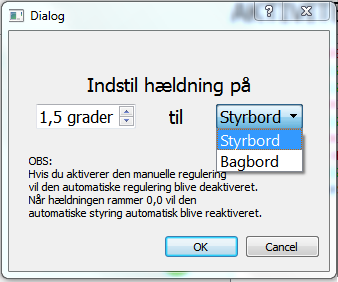
\includegraphics[scale=1]{billeder/GUI/manuelvindue}
\label{fig:manuelvindue}
\caption{På figuren ses vinduet for manuel indstilling af vinkel}
\end{figure}

\section*{Automatisk regulering af hældning}
Ved tryk på knappen med teksten "AKTIVER AUTOMATISK HÆLDNINGSREGULERING" (boks syv på figur \ref{fig:hovedvindue}) kommer en dialog frem. Såfremt automatisk hældnings allerede er aktiveret (som indikeret med en grøn cirkel øverst i boks fem på figur \ref{fig:hovedvindue}) fremkommer dialogen på figur \ref{fig:auto_accept} frem.
Hvis automatisk hældning ikke er aktiveret fremkommer dialogen på figur \ref{fig:auto_denial} frem.

\begin{figure}[h]
\centering
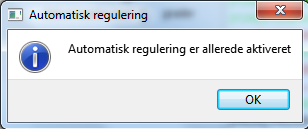
\includegraphics[scale=0.8]{billeder/GUI/auto_aktiveret}
\label{fig:auto_accept}
\caption{Ved tryk på AKTIVER AUTOMATISK HÆLDNINGSREGULERING når automatisk hældningsregulering allerede er aktiveret}
\end{figure}

\begin{figure}[h]
\centering
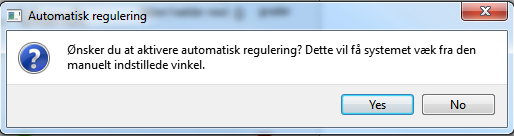
\includegraphics[scale=0.8]{billeder/GUI/aktiver_auto}
\label{fig:auto_denial}
\caption{Ved tryk på knappen i boks syv på figur \ref{fig:hovedvindue} når automatisk hældningsregulering ikke er aktiveret}
\end{figure}

\section*{Termineringsdialog}
Denne advarsel fremkommer når man trykker på knappen i boks to på figur \ref{fig:hovedvindue}.

\begin{figure}[h]
\centering
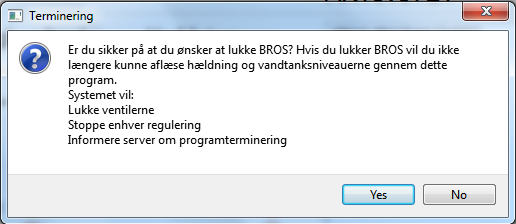
\includegraphics[scale=0.8]{billeder/GUI/termineringsvindue}
\label{fig:terminering}
\caption{Advarsel før nedlukning af BROS}
\end{figure}